\documentclass{article}
\usepackage{tikz}
\usepackage{pgfplots}
\usepackage{xcolor}
\usepackage{svg}
\usepackage{amsmath}
\usepackage{array}
\usepackage[skins]{tcolorbox}
\usepackage[version=4]{mhchem}
\usepackage[a4paper, total={6in, 9in}]{geometry}
\usepackage{fourier}
\usepackage{xymtex}
\usepackage{textcomp}
\usepackage{eurosym}
\usepackage{caption}
\usepackage{longtable}
\usepackage{float}
\usepackage{attachfile}
\usepackage{multirow}

\captionsetup[table]{name=\textit{Tabella}}
\pagenumbering{gobble}
\setcounter{secnumdepth}{2}

\title{Relazione di laboratorio - Esperienza di Poisson}
\author{Federico Cesari}
\date{Marzo 2024}




\begin{document}
\begin{titlepage}
	\begin{center}
		\vspace*{1cm}
		
		\textbf{\LARGE Relazione di laboratorio - Pendolo semplice}
		
		\vspace{0.3cm}
		\large \textit{Misura del periodo di un pendolo semplice} \\
		
		\vspace{0.5cm}
		\Large Federico Cesari \\
		
		\small 1096759 
		\vspace{0.2cm}
		
		\small Gruppo 5
		
		
		\vspace{3cm}
		\begin{center}
			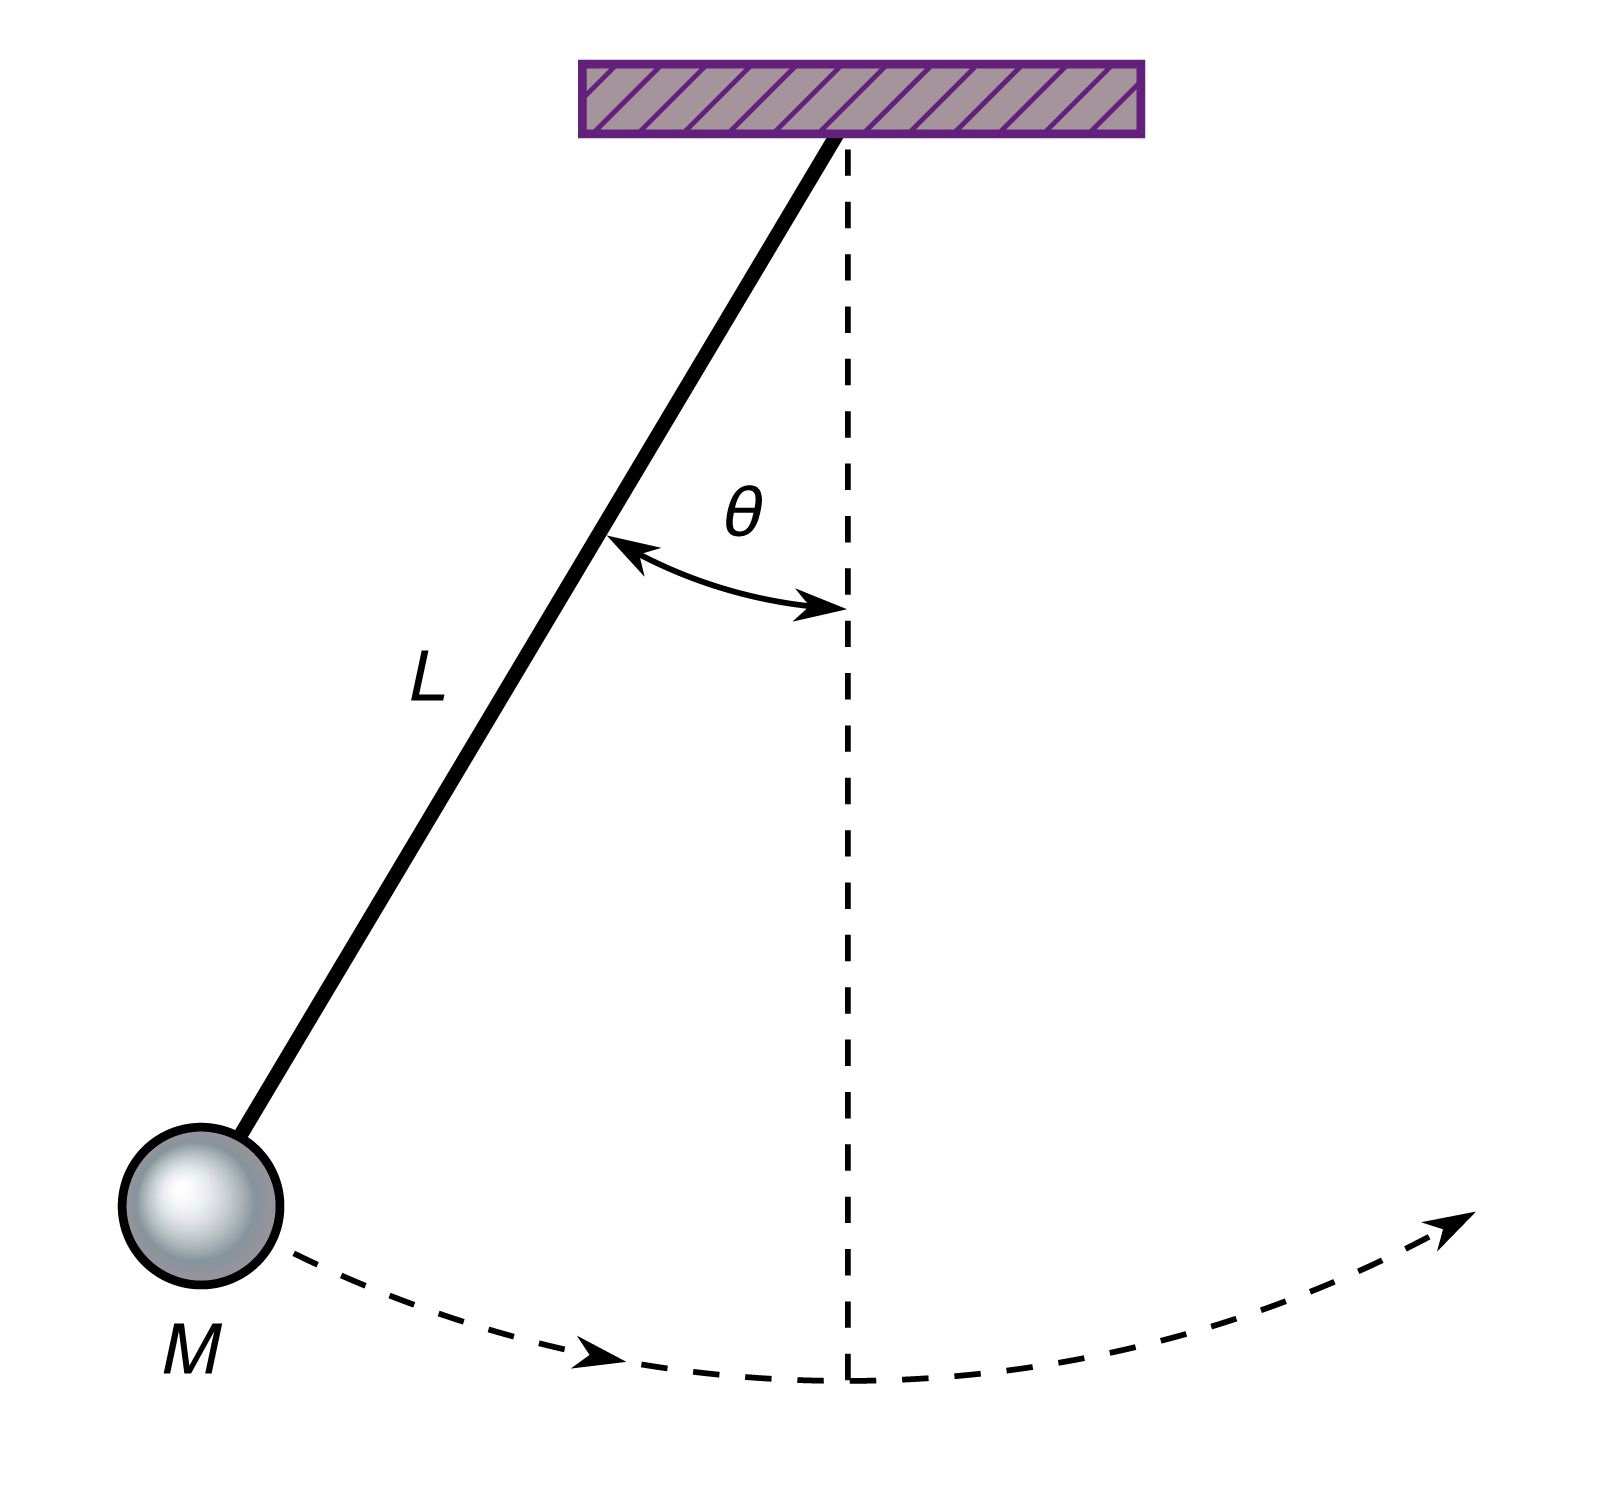
\includegraphics[scale=0.1]{IMG_0200.jpeg}	
		\end{center}
		
		
		
		\vfill
		
		
		
		corso A\\
		Università degli studi di Torino, Torino\\
		4 aprile 2024\\
		
		
	\end{center}
\end{titlepage}

%Scopo : misurare il rate 
%rilevatore di radiazioni: contatore geiger
%rotaia con uranile a 3cm

%Calcolare il rate del fondo: rapporto tra media e deviazione standard e tempo porta.

%\section{Test $\chi^2$}
%!incertezza per somma e differenza è la radice quadrata della somma dei quadrati delle incertenza. 
%\begin{enumerate}
%	\item 	rate fondo (tempo porta = 1s): $RF(1sec) = 0.305 \pm 0.014 s^{-1}$. (\textit{nonost			   ante preferisca una sola cifra significativa per l'errore lascio 0.014, sottostimer			      ei di troppo se arrotondassi}.)
%	\item rate fondo + sorgente (tempo porta = 1s): $RFS(<1sec) = 3.145 \pm 0.045 s^{-1}$
%\end{enumerate}
%\[
%RS(1sec) = RFS(1sec) - RF(1sec) 
%\]

%con errore
%\[
%\delta_{RS(1sec)} =\sqrt{\delta_{RFS(1sec)}^2 + \delta_{RF(1sec)}^2}
%\]

\section{Scopo dell'esperienza}
L'esperienza di laboratorio ha come scopo la misurazione del rate di una sorgente radioattiva, ovvero il numero di eventi registrati in tempi porta di $1$ e $3$ secondi dal contatore geiger quando la sorgente è posta a \(3\)cm da questo. \\

\noindent
L'apparato sperimentale utilizzato consiste di: un rilevatore di radiazione (contatore geiger) posto su una rotaia e una pietra di uranile utilizzata come sorgente radioattiva.

\section{Acquisizione dati}
Prima di effettuare le misurazioni del rate della sorgente radioattiva misuro il rate dovuto solamente alla radioattività naturale di fondo. La radiazione di fondo è causata dalla presenza di gas radioattivi come Radon e Torio in atmosfera, dalla presenza di elementi radioattivi nel terreno e in acqua, oppure da radiazioni cosmiche che portano  particelle ad alta energia cariche positivamente che entrano in atmosfera provocando l'emissione di fotoni, elettroni e neutroni. 

Nel momento in cui dovrò misurare il rate dell'uranile dovrò tenere in considerazione la presenza dei conteggi dovuti al fondo.


\vfill
% FONDO
\section{Distribuzione sperimentale del fondo}
Senza avvicinare la sorgente radioattiva al contatore geiger prendo 1500 misurazioni, prima con tempo porta di 1s e poi di 3s, del rate della radiazione di fondo.


%ISTOGRAMMI 1
\vspace{0.5cm}
\hspace{-0.7cm}
\begin{minipage}[c]{0.45\textwidth}
\begin{center}
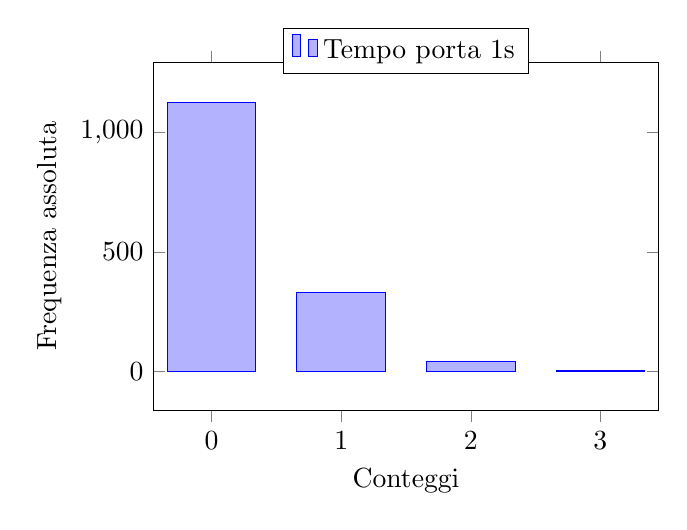
\begin{tikzpicture}
\pgfplotsset{compat = 1.3}
\begin{axis}[
	width=8cm, 
	height=6cm,
	ylabel=Frequenza assoluta,
	xlabel=Conteggi,
	enlargelimits=0.15,
	legend style={at={(0.5,1.1)},	anchor=north,legend columns=-1},
	ybar=0pt,% configures `bar shift'
	bar width=32pt,
	xtick={0,1,2,3},
	xticklabels={0,1,2,3},
	xticklabel style={rotate=0,align=center}]
	\addplot+[opacity=1] 
	coordinates {
		(0,1125)
		(1,330)
		(2,41)
		(3,4)};
	\legend{Tempo porta 1s}
\end{axis}
\end{tikzpicture}
\end{center}
\end{minipage}
\hfill
\begin{minipage}[c]{0.45\textwidth}
\begin{center}
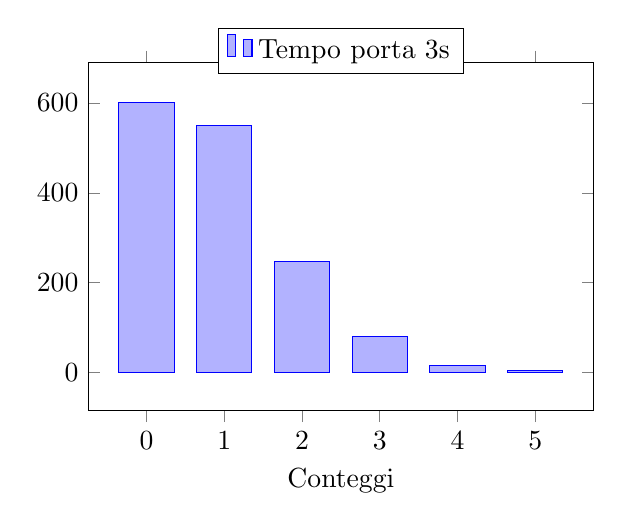
\begin{tikzpicture}
\pgfplotsset{compat = 1.3}
\begin{axis}[
	width=8cm, 
	height=6cm,
	xlabel=Conteggi,
	enlargelimits=0.15,
	legend style={at={(0.5,1.1)},	anchor=north,legend columns=-1},
	ybar=0pt,% configures `bar shift'
	bar width=20pt,
	xtick={0,1,2,3,4,5},
	xticklabels={0,1,2,3,4,5},
	xticklabel style={rotate=0,align=center}]
	\addplot+[opacity=1] 
	coordinates {
		(0,601)
		(1,551)
		(2,247)
		(3,81)
		(4,15)
		(5,5)};
	\legend{Tempo porta 3s}
\end{axis}
\end{tikzpicture}
\end{center}
\end{minipage}


%TABELLE 1
\begin{minipage}[c]{0.45\textwidth}
\vspace{1cm}
\begin{center}
\hspace{0.5cm}
\begin{tabular}{llr}
	Media                       & $\bar{x}$             & $0.283$       \\		
	Varianza                    & $\sigma_{x}^2$          & $0.274$     \\
	Dev. std                    & $\sigma_{x}$              & $0.523$   \\
	Dev. std (della media)      & $\sigma_{\bar{x}}$    & $0.014$       \\
\end{tabular}
\captionof{table}{\textit{Tempo porta 1s}}
\end{center}

\[ 
	\text{\textbf{Rate del fondo (1s)}} = 0.283 \text{ count/s}
\]
\end{minipage}
\hfill
\begin{minipage}[c]{0.45\textwidth}
\vspace{1cm}
\begin{center}
\begin{tabular}{llr}
	Media                       & $\bar{x}$             & $0.915$       \\		
	Varianza                    & $\sigma_{x}^2$          & $0.918$     \\
	Dev. std                    & $\sigma_{x}$              & $0.958$   \\
	Dev. std (della media)      & $\sigma_{\bar{x}}$    & $0.025$       \\
\end{tabular}
\captionof{table}{\textit{Tempo porta 3s}}
\end{center}

\[ 
	\text{\textbf{Rate del fondo (3s)}} = 0.305 \text{ count/s}
\]
\end{minipage}




% FONDO + SORGENTE    3cm
\section{Distribuzione sperimentale di fondo + sorgente a 3cm}
Posizionata la pietra di uranile a 3cm dal contatore prendo 1500 misurazioni 

\vspace{0.6cm}
\begin{minipage}[c]{0.5\textwidth}
\begin{center}
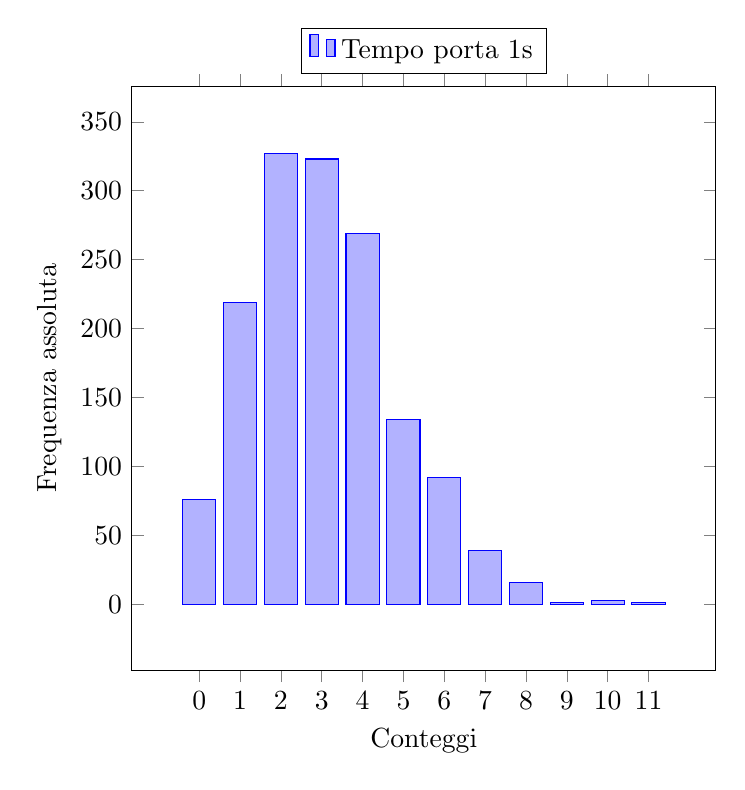
\begin{tikzpicture}
\pgfplotsset{compat = 1.3}
\begin{axis}[
	width=9cm, 
	height=9cm,
	ylabel=Frequenza assoluta,
	xlabel=Conteggi,
	enlargelimits=0.15,
	legend style={at={(0.5,1.1)},	anchor=north,legend columns=-1},
	ybar=0pt,  % configures `bar shift'
	bar width=12pt,
	xtick={0,1,2,3,4,5,6,7,8,9,10,11},
	xticklabels={0,1,2,3,4,5,6,7,8,9,10,11},
	xticklabel style={rotate=0, align=center}]
	\addplot+[opacity=1] 
	coordinates {
		(0,76)
		(1,219)
		(2,327)
		(3,323)
		(4,269)
		(5,134)
		(6,92)
		(7,39)
		(8,16)
		(9,1)
		(10,3)
		(11,1)};
	\legend{Tempo porta 1s}
\end{axis}
\end{tikzpicture}
\end{center}
\end{minipage}
\hfill
\begin{minipage}[c]{0.4\textwidth}
\begin{center}
\begin{tabular}{llr}
	Media                       & $\bar{x}$             & $3.061$       \\		
	Varianza                    & $\sigma_{x}^2$          & $3.192$     \\
	Dev. std                    & $\sigma_{x}$              & $1.787$   \\
	Dev. std (della media)      & $\sigma_{\bar{x}}$    & $0.046$       \\
\end{tabular}
\captionof{table}{\textit{1500}}
\end{center}
\vspace{1cm}
\[ 
	\text{\textbf{Rate del fondo + sorgente }}
\]
\[
	\mathbf{= \left(3.061 \pm 0.046\right)} \text{ \textbf{count/s}}
\]
\end{minipage}

\vfill

\begin{minipage}[c]{0.4\textwidth}
\begin{center}
\begin{tabular}{llr}
	Media                       & $\bar{x}$             & $9.343$       \\		
	Varianza                    & $\sigma_{x}^2$          & $9.562$     \\
	Dev. std                    & $\sigma_{x}$              & $3.092$   \\
	Dev. std (della media)      & $\sigma_{\bar{x}}$    & $0.080$       \\
\end{tabular}
\captionof{table}{\textit{1500}}
\end{center}
\vspace{1cm}
\[ 
	\text{\textbf{Rate del fondo + sorgente }}
\]
\[
	\mathbf{=  \left(3.114 \pm 0.027\right)} \text{ \textbf{count/s}}
\]
\end{minipage}
\hfill
\begin{minipage}[c]{0.6\textwidth}
\begin{center}
\begin{tikzpicture}
\pgfplotsset{compat = 1.3}
\begin{axis}[
	width=10cm, 
	height=10cm,
	ylabel=Frequenza assoluta,
	xlabel=Conteggi,
	enlargelimits=0.15,
	legend style={at={(0.5,1.1)},	anchor=north,legend columns=-1},
	ybar=0pt,  % configures `bar shift'
	bar width=10pt,
	xtick={0,1,2,3,4,5,6,7,8,9,10,11,12,13,14,15,16,17,18,19,20,21},
	xticklabels={0,\tiny{1},2,\tiny{3},4,\tiny{5},6,\tiny{7},8,\tiny{9},10,\tiny{11},12,\tiny{13},14,\tiny{15},16,\tiny{17},18,\tiny{19},20,\tiny{21}},
	xticklabel style={rotate=0, align=center},
	ytick pos=right]
	\addplot+[opacity=1] 
	coordinates {
		(0,0)
		(1,0)
		(2,5)
		(3,17)
		(4,34)
		(5,77)
		(6,127)
		(7,192)
		(8,195)
		(9,181)
		(10,184)
		(11,143)
		(12,107)
		(13,92)
		(14,60)
		(15,31)
		(16,30)
		(17,8)
		(18,7)
		(19,6)<LeftMouse>
		(20,3)
		(21,1)};
	\legend{Tempo porta 3s}
\end{axis}
\end{tikzpicture}
\end{center}
\end{minipage}






% CHI QUADRO
\newpage
\section{Test \(\chi^2\)}
\subsection{Test \(\chi^2\) con tempo porta di 1s}
Tramite il test del \(\chi^2\) verifico se le distribuzioni teoriche di Poisson e di Gauss si adattano a quelle sperimentali calcolate con tempo porta di 1 secondo.

Scelgo un livello di significatività $\alpha = 5\%$ e calcolo i rispettivi $\chi^2$ critici e i gradi di libertà.


\subsubsection{Adattamento a Poissoniana (1s)}
\paragraph{Ipotesi nulla} La distribuzione teorica di Poisson si adatta alla distribuzione sperimentale.

\vspace{0.2cm}
\begin{center}
\begin{tabular}{lr}
	Numero classi & $10$ \\
	Livello di significatività $\alpha$		& $ \quad 5\%$  \\
	Valore di $\chi ^2$             	& $\quad 8.813$       \\
	Numero di gradi di libertà      	& $\quad (10-1-1) = 8$         \\   
	Valore di $\chi ^2$ critico     	& $\quad 15.507$
\end{tabular}
\captionof{table}{\textit{$\chi^2$ Poissoniana}}
\end{center}

\paragraph{Coclusione del test} Poiché $\chi^2 < \chi^2_{\text{critico}}$, la discrepanza tra le frequenze attese e quelle osservate risulta essere accettabile nei livelli di significatività scelti. Posso dire che la distribuzione teorica di Poisson si adatta bene alla distribuzione sperimentale e quindi \textbf{accetto} l'ipotesi nulla.


\subsubsection{Adattamento a Gaussiana (1s)}
\paragraph{Ipotesi nulla} La distribuzione teorica di Gauss si adatta alla distribuzione sperimentale.

\vspace{0.2cm}
\begin{center}
\begin{tabular}{lr}
	Numero classi & $11$ \\
	Livello di significatività $\alpha$		& $ \quad 5\%$  \\
	Valore di $\chi ^2$             	& $\quad 96.060$       \\
	Numero di gradi di libertà      	& $\quad (11-2-1) = 8$         \\   
	Valore di $\chi ^2$ critico     	& $\quad 15.507$
\end{tabular}
\captionof{table}{\textit{$\chi^2$ Poissoniana}}
\end{center}

\paragraph{Coclusione del test} Poiché $\chi^2 > \chi^2_{\text{critico}}$ la discrepanza tra le frequenze attese e quelle osservate supera i valori accettabili nei livelli di significatività scelti. Posso dire che la distribuzione teorica di Gauss non si adatta alla distribuzione sperimentale e quindi \textbf{rifiuto} l'ipotesi nulla.

\begin{center}
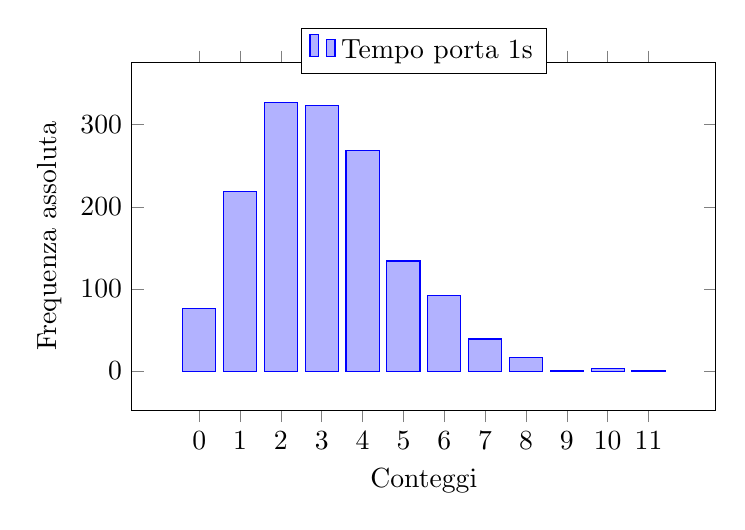
\begin{tikzpicture}
\pgfplotsset{compat = 1.3}
\begin{axis}[
	width=9cm, 
	height=6cm,
	ylabel=Frequenza assoluta,
	xlabel=Conteggi,
	enlargelimits=0.15,
	legend style={at={(0.5,1.1)},	anchor=north,legend columns=-1},
	ybar=0pt,  % configures `bar shift'
	bar width=12pt,
	xtick={0,1,2,3,4,5,6,7,8,9,10,11},
	xticklabels={0,1,2,3,4,5,6,7,8,9,10,11},
	xticklabel style={rotate=0, align=center}]
	\addplot+[opacity=1] 
	coordinates {
		(0,76)
		(1,219)
		(2,327)
		(3,323)
		(4,269)
		(5,134)
		(6,92)
		(7,39)
		(8,16)
		(9,1)
		(10,3)
		(11,1)};
	\legend{Tempo porta 1s}
\end{axis}
\end{tikzpicture}
\end{center}


\subsection{Test \(\chi^2\) con tempo porta di 3s}
Tramite il test del \(\chi^2\) verifico se le distribuzioni teoriche di Poisson e di Gauss si adattano a quelle sperimentali calcolate con tempo porta di 1 secondo.

Scelgo un livello di significatività $\alpha = 5\%$ e calcolo i rispettivi $\chi^2$ critici e i gradi di libertà.


\subsubsection{Adattamento a Poissoniana (3s)}
\paragraph{Ipotesi nulla} La distribuzione teorica di Poisson si adatta alla distribuzione sperimentale.

\vspace{0.2cm}
\begin{center}
\begin{tabular}{lr}
	Numero classi & $17$ \\
	Livello di significatività $\alpha$		& $ \quad 5\%$  \\
	Valore di $\chi ^2$             	& $\quad 19.371$       \\
	Numero di gradi di libertà      	& $\quad (17-1-1) = 15$         \\   
	Valore di $\chi ^2$ critico     	& $\quad 24.996$
\end{tabular}
\captionof{table}{\textit{$\chi^2$ Poissoniana}}
\end{center}

\paragraph{Coclusione del test} Poiché $\chi^2 < \chi^2_{\text{critico}}$, la discrepanza tra le frequenze attese e quelle osservate risulta essere accettabile nei livelli di significatività scelti. Posso dire che la distribuzione teorica di Poisson si adatta bene alla distribuzione sperimentale e quindi \textbf{accetto} l'ipotesi nulla.


\subsubsection{Adattamento a Gaussiana (3s)}
\paragraph{Ipotesi nulla} La distribuzione teorica di Gauss si adatta alla distribuzione sperimentale.

\vspace{0.2cm}
\begin{center}
\begin{tabular}{lr}
	Numero classi & $18$ \\
	Livello di significatività $\alpha$		& $ \quad 5\%$  \\
	Valore di $\chi ^2$             	& $\quad 59.344$       \\
	Numero di gradi di libertà      	& $\quad (18-2-1) = 15$         \\   
	Valore di $\chi ^2$ critico     	& $\quad 24.966$
\end{tabular}
\captionof{table}{\textit{$\chi^2$ Poissoniana}}
\end{center}

\paragraph{Coclusione del test} Poiché $\chi^2 > \chi^2_{\text{critico}}$ la discrepanza tra le frequenze attese e quelle osservate supera i valori accettabili nei livelli di significatività scelti. Posso dire che la distribuzione teorica di Gauss non si adatta alla distribuzione sperimentale e quindi \textbf{rifiuto} l'ipotesi nulla.


\begin{center}
\begin{tikzpicture}
\pgfplotsset{compat = 1.3}
\begin{axis}[
	width=10cm, 
	height=7cm,
	ylabel=Frequenza assoluta,
	xlabel=Conteggi,
	enlargelimits=0.15,
	legend style={at={(0.5,1.1)},	anchor=north,legend columns=-1},
	ybar=0pt,  % configures `bar shift'
	bar width=10pt,
	xtick={0,1,2,3,4,5,6,7,8,9,10,11,12,13,14,15,16,17,18,19,20,21},
	xticklabels={0,\tiny{1},2,\tiny{3},4,\tiny{5},6,\tiny{7},8,\tiny{9},10,\tiny{11},12,\tiny{13},14,\tiny{15},16,\tiny{17},18,\tiny{19},20,\tiny{21}},
	xticklabel style={rotate=0, align=center}]
	\addplot+[opacity=1] 
	coordinates {
		(0,0)
		(1,0)
		(2,5)
		(3,17)
		(4,34)
		(5,77)
		(6,127)
		(7,192)
		(8,195)
		(9,181)
		(10,184)
		(11,143)
		(12,107)
		(13,92)
		(14,60)
		(15,31)
		(16,30)
		(17,8)
		(18,7)
		(19,6)<LeftMouse>
		(20,3)
		(21,1)};
	\legend{Tempo porta 3s}
\end{axis}
\end{tikzpicture}
\end{center}


\newpage
\subsection{Test di Gauss}
Tramite il Test Z stabilisco se il rate calcolato per tempo porta di 1s è compatibile con il rate calcolato per tempo porta di 3s.


\end{document}
